\documentclass[11pt, a4paper]{article}

\usepackage{graphicx}
\usepackage[a4paper,top=3cm,bottom=2cm,left=2cm,right=2cm,marginparwidth=1.75cm]{geometry}
\usepackage[english]{babel}
\usepackage[utf8x]{inputenc}
\usepackage{subfig}
\usepackage{amsmath}
\usepackage{amssymb}

\graphicspath{ {./images} }
\newcommand*{\qed}{\hfill\ensuremath{\quad\square}}%
\newcommand*{\rad}{\ensuremath{\,\text{rad}}}
\newcommand*{\R}{\ensuremath{\mathbb{R}}}

\makeatletter
\renewcommand*\env@matrix[1][*\c@MaxMatrixCols c]{%
  \hskip -\arraycolsep
  \let\@ifnextchar\new@ifnextchar
  \array{#1}}
\makeatother

\newtheorem{theorem}{Theorem}

%------------------------------------------------
%Templates for images and figures
% \begin{figure}[h]
%   \centering
%   \subfloat[caption 1]{{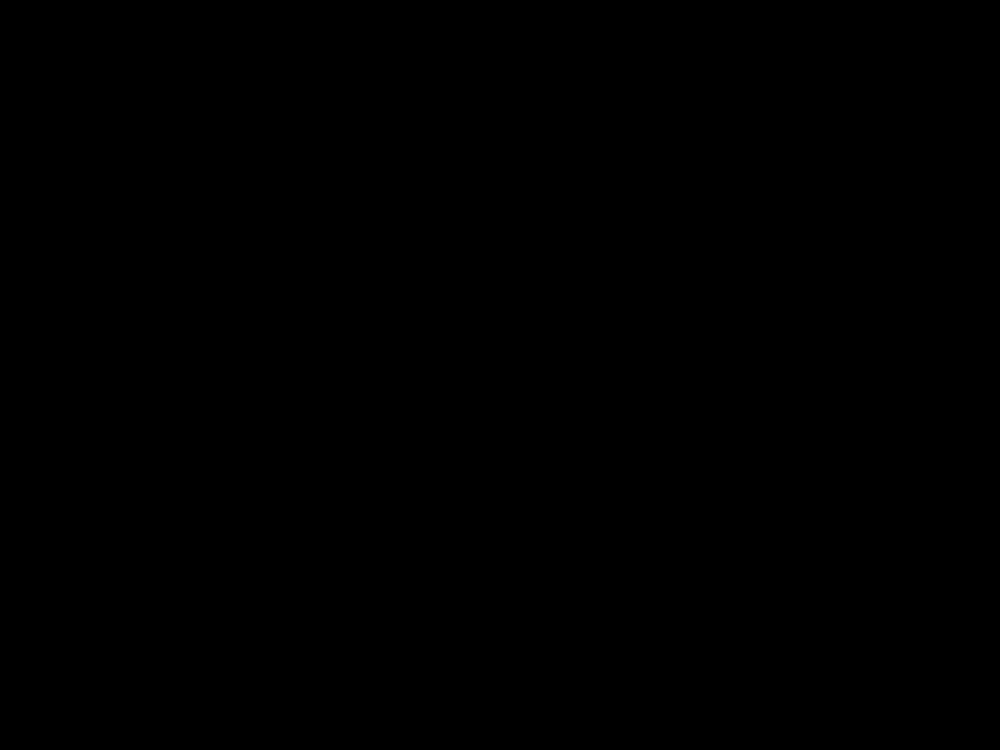
\includegraphics[width=30mm]{images/placeholder.png}}}%
%   \qquad
%   \subfloat[caption 2]{{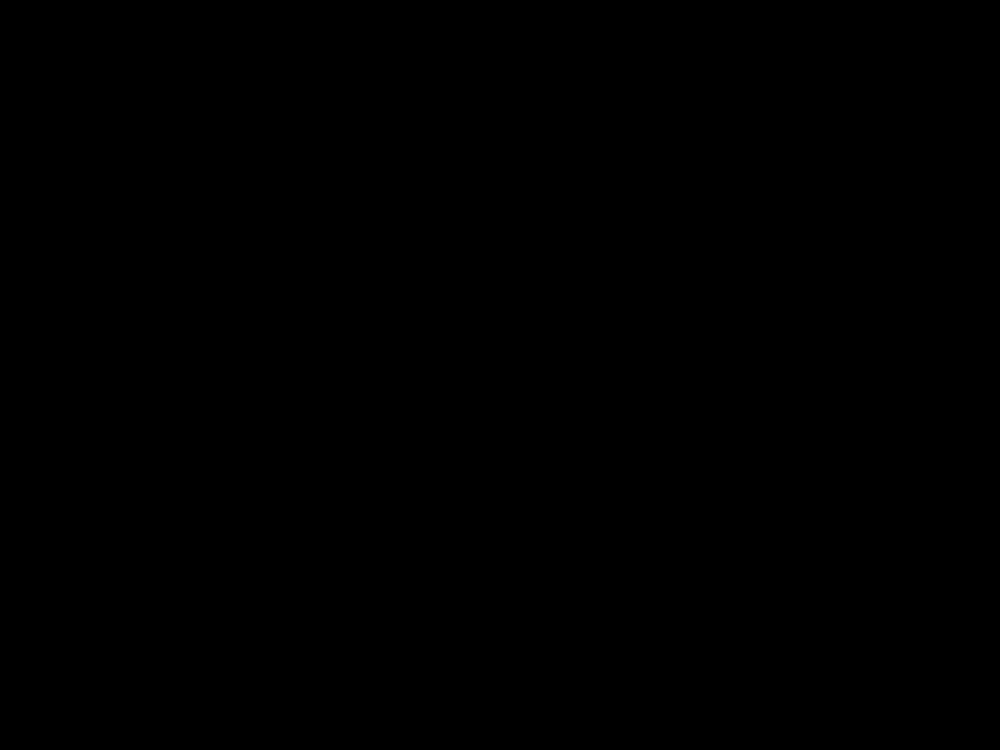
\includegraphics[width=30mm]{images/placeholder.png}}}%
%   \caption{Description}
% \end{figure}

% \begin{figure}[h]
%   \centerline{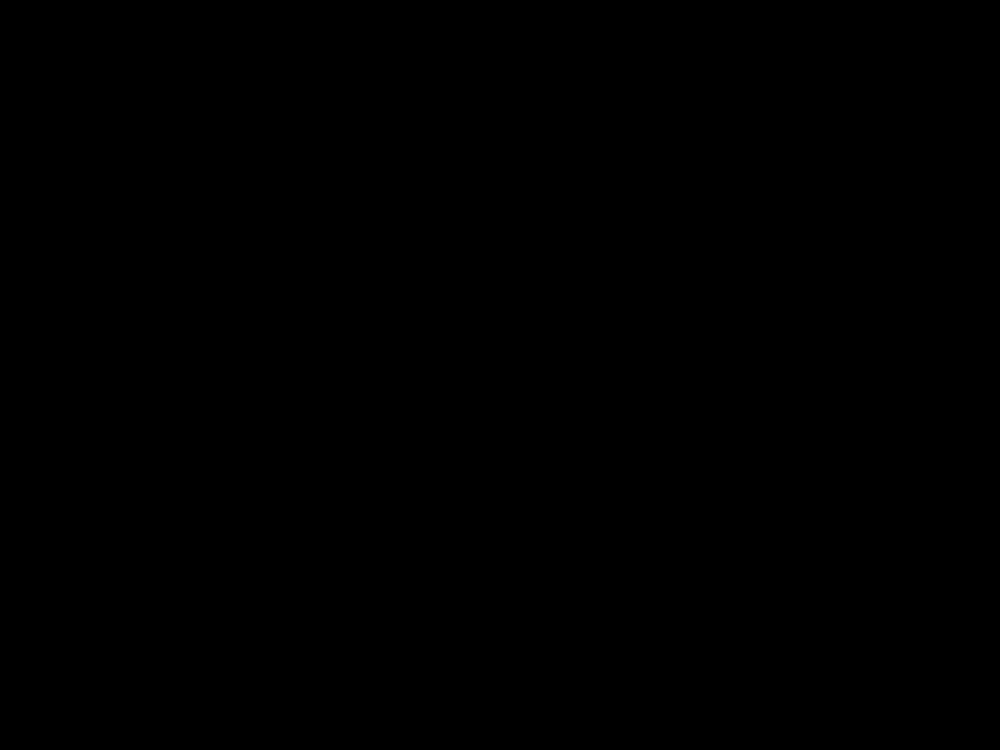
\includegraphics[width=50mm]{images/placeholder.png}}
%   \caption{Description}
% \end{figure}
%-----------------------------------------------

\begin{document}
\setcounter{section}{1}
\setcounter{equation}{0}

\section{Thermofluids Lecture 2: First law of thermodynamics (23/04/2020)}


\subsection{The first law for a closed system}
The first law of thermodynamics states the following: Energy can be transformed from one form to another, however it cannot be created or destroyed. The first law of thermodynamics for a closed system takes the following form\footnote{Sometimes also written as $Q + W$ rather then $Q - W$, but this is just a sign convention depending on which direction of work is taken to be positive.}:
\begin{equation}
  \Delta KE + \Delta PE + \Delta U = Q - W
\end{equation}
Where $\Delta KE$ is the kinetic energy, $\Delta PE$ is the potential energy, $\Delta U$ the internal energy and $\Delta E$ the change in the total energy of the system.\\
Energy can be transferred from and into a system in 3 forms: heat transfer $Q$, work transfer $W$ and mass flow $m$. Thus the total differnce in energy is described as:
\begin{equation}
  \Delta E_{system} = E_{in} - E_{out} = (Q_{in} - Q_{out}) + (W_{in} - W_{out}) + (E_{mass,in} - E_{mass,out})
\end{equation}
Where the subscripts $in$ and $out$ denote the quantities that enter and leave the system. This subscript can be thought of as the direction of the energy. The flow of energy in a system can also be expressed as a flow rate by taking the time derrivative of the previous expression:
\begin{equation}
  \frac{dE_{system}}{dt} = \dot{E}_{in} - \dot{E}_{out}
\end{equation}
For a closed system there is no transfer of mass going into or out of the system. Thus the expression becomes:
\begin{equation}
  \frac{dE_{system}}{dt} = \dot{Q} - \dot{W}
\end{equation}

\subsection{Internal energies of a system}
The internal energies of a system are a microscopic phenomena. Examples of this are kinetic energy of atoms (translational and rotational), vibrations of atoms, chemical energies, nuclear energy, lattice energy, etc. Though statisical mechanics has gone a long way in explaining the exact nature of these internal energy we usually do not concern ourselfs with these in classical thermodynamics. The internal energy of a system in differential form can be written as:
\begin{gather}
  dU = \delta Q - \delta W
\end{gather}
The internal energy can be expressed on a macroscopic scale with the following equation. Note that this heavily simplified:
\begin{equation}
  U = Cm \Delta T
\end{equation}
Where $C$ is the heat capacity at constant volume. 

\subsection{Heat and work in thermodynamics}
Mechanical work done is usually described with the following integral:
\begin{equation}
  W = \int_{s1}^{s2} \vec{F}\cdot d\vec{s}
\end{equation}
The understanding of work needs to be extended a bit for thermodynamics. In thermodynamics any energy interaction not caused by a difference in temperature is considered work. Thus electrical energy entering a system can be considered work. However note that work is a process variable. This holds for all types of work in thermodynamics. Because of this the following integral can only be eveluated when some details about the process are known, which is not the case for classical thermodynamics:
\begin{equation}
  W = \int_1^2 \delta W
\end{equation}
Where the $\delta$ is used to denote an inexact differential. Using this $\delta$ automatically implies path dependence. Note the expression for the first law where the LHS contains only state variables, while the RHS only contains process variables. This idea of inexact differentials applies to all process variables. Thus the total differential difference in energy of a system can be expressed as:
\begin{equation}
  \delta E_{in} - \delta E_{out} = dE_{system}
\end{equation}
For a system undergoing a cycle we can state that $\Delta E_{system} = 0\,J$. This leads to the following conclusion:
\begin{equation}
  W_{net,out} = Q_{net,in}
\end{equation}


\subsection{Modeling expansion or compression work}
Consider a cylinder with a volume $V$. The gas inside this cylinder has a pressure $p$ and the piston has an area $A$. The force acting on the piston can then be described as:
\begin{equation}
  F = pA\\
\end{equation}
The work done by the system can then be formulated as follows:
\begin{gather}
  \delta W_{12} = F\,ds = pA\,dx = p\,dV\\
  W = \int_{V_1}^{V_2} p\,dV
\end{gather}
Note that the previous integral can be evaluated because it is only dependent on state variables (in this case Volume). By sign convention this is negative work if the volume increases since this is work done by the system itself. When the volume decreases this is work done on the system thus increasing the total energy. 
\begin{gather}
  \delta W = p\,dV \quad \text{and} \quad dU = mc\,dT\\
  -\delta W = dU\\
  -p\,dV = dU
\end{gather}
\begin{figure}[h!]
  \centerline{\includegraphics[width=50mm]{images/Work Done.png}}
  \caption{Situation of the moving piston}
\end{figure}
\end{document}